\documentclass[a4paper, oneside]{memoir}
\usepackage[utf8]{inputenc}
\usepackage[T1]{fontenc}
\usepackage{pifont}
\usepackage{amssymb}
\usepackage{fourier}
\usepackage[dvipsnames]{xcolor}
\usepackage{tikz}
\usepackage{pdfpages}
\usepackage[sfdefault]{roboto}
\usepackage{color}

\tikzstyle{teamshare} = [below, text width=5.4cm, inner sep = 0.5cm, text=white, align=center]
\tikzstyle{cardtext} = [below, text width=5.9cm, inner sep = 0.25cm, text centered]

% Define Commands
\newcommand{\condition}[1]{\textbf{#1}}
\newcommand{\character}[1]{\textbf{#1}}
\newdimen\titlespacing
\titlespacing=0.15cm

% Define Seperators
\newcommand{\redseperator}{\vspace{\titlespacing} \hrulefill {} \ding{100} \hrulefill\\ \vspace{\titlespacing}}
\newcommand{\greenseperator}{\vspace{\titlespacing} \hrulefill {} \bomb{}/\ding{72} \hrulefill\\ \vspace{\titlespacing}}
\newcommand{\greyseperator}{\vspace{\titlespacing} \hrulefill {} \ding{100} \hrulefill\\ \vspace{\titlespacing}}
\newcommand{\purpleseperator}{\vspace{\titlespacing} \hrulefill {} \bomb{}/\ding{72} \hrulefill\\ \vspace{\titlespacing}}
\newcommand{\actionseperator}{\vspace{\titlespacing} \hrulefill {} \tiny power \normalsize \hrulefill\\ \vspace{\titlespacing}}
\newcommand{\descriptionseperator}{\vspace{\titlespacing} \hrulefill {} \tiny description \normalsize \hrulefill\\ \vspace{\titlespacing}}
\newcommand{\modifierseperator}{\vspace{\titlespacing} \hrulefill {} \tiny power \normalsize \hrulefill\\ \vspace{\titlespacing}}
\newcommand{\conditionseperator}{\vspace{\titlespacing} \hrulefill {} \tiny condition \normalsize \hrulefill\\ \vspace{\titlespacing}}
\newcommand{\winseperator}{\vspace{\titlespacing} \hrulefill {} \tiny how to win \normalsize \hrulefill\\ \vspace{\titlespacing}}
\newcommand{\redwinsection}{
	\winseperator
	You win if \character{Santa} does not gain the \condition{humbug} condition due to the \character{Grinch} stealing Christmas.
}
\newcommand{\greenwinsection}{
	\winseperator
	\small You win if \character{Santa} gains the \condition{humbug} condition due to the \character{Grinch} stealing Christmas.
}

%Margin-indstillinger:
\setlrmarginsandblock{0.9cm}{*}{1} %angiver venstre-, så højremargin
\setulmarginsandblock{1.49cm}{*}{1} %angiver øvre-, så nedremargin
\checkandfixthelayout[nearest]

%Følgende giver en minimal sidehoved og sidefod hvor der kun er sidetal.
\pagestyle{empty}

\begin{document}
\noindent 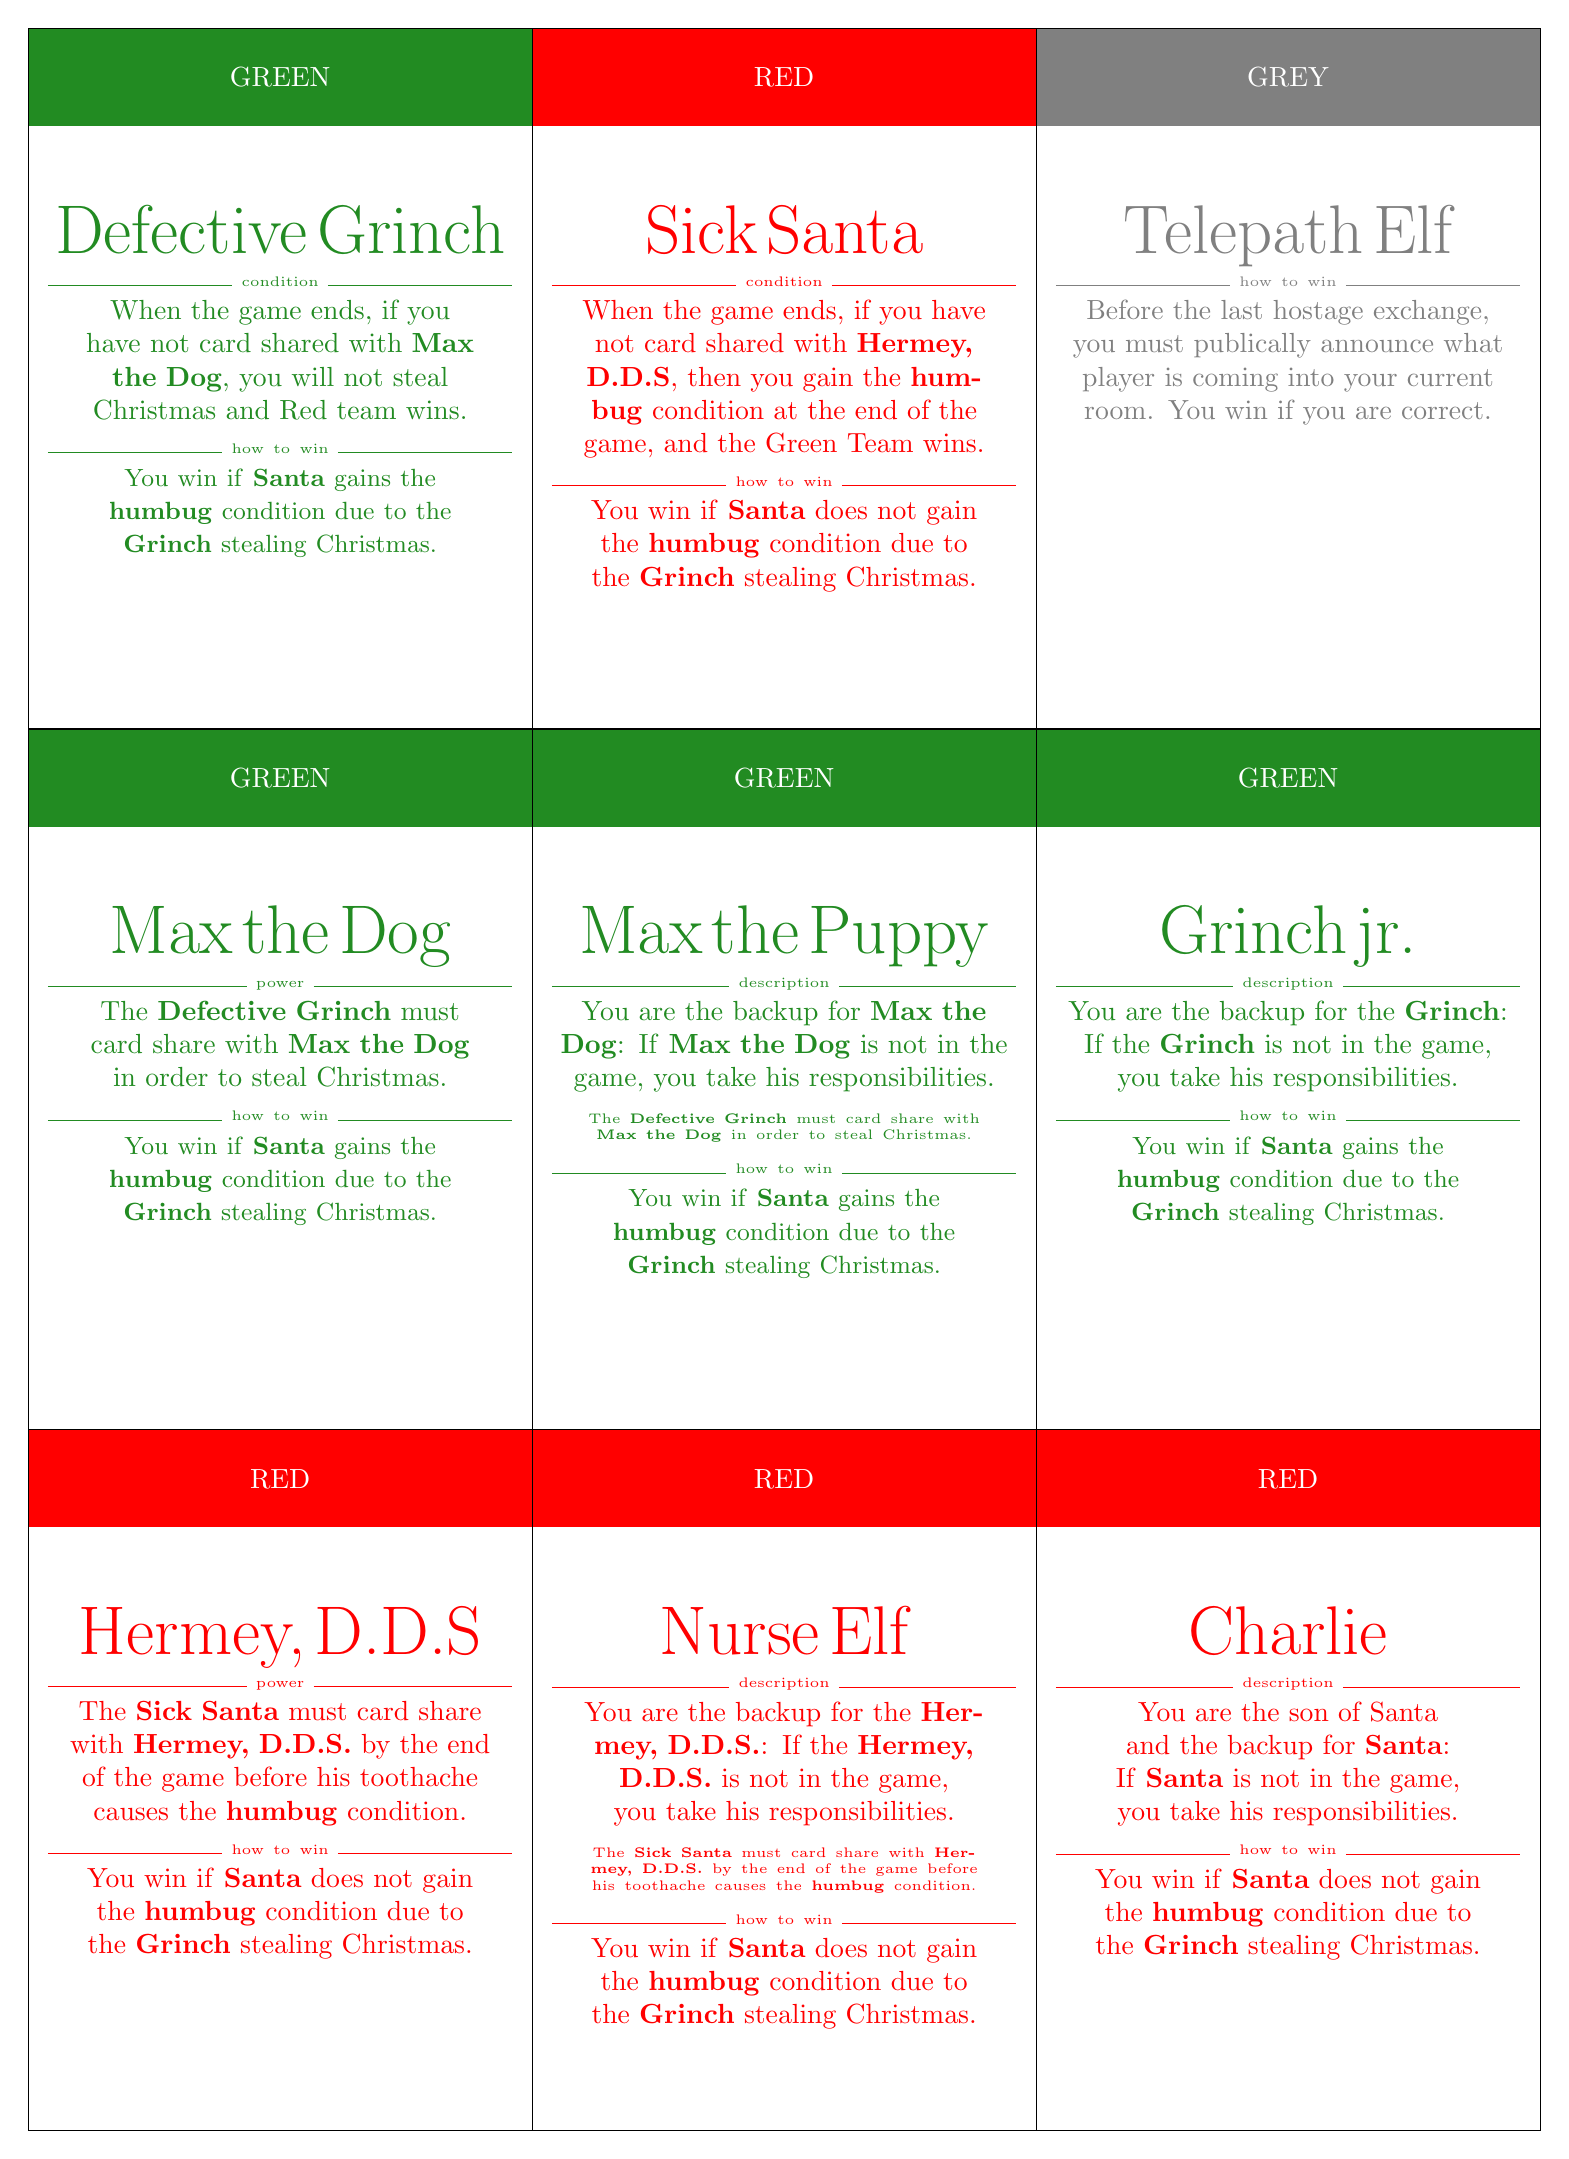
\begin{tikzpicture}[outer sep=0]

% DEFECTIVE GRINCH
\node[teamshare, fill=ForestGreen] (1) at (3.2,26.7) {\HUGE GREEN};
\node[cardtext, text=ForestGreen] at (3.2,24.7) {
	{\Huge Defective Grinch}
	\\\conditionseperator
	When the game ends, if you have not card shared with \character{Max the Dog}, you will not steal Christmas and Red team wins.
	\\\vspace{0.01cm}
	\greenwinsection
};

% SICK SANTA
\node[teamshare, fill=red] at (9.6,26.7) {\HUGE RED};
\node[cardtext, text=red] at (9.6,24.7) {
	{\Huge Sick Santa}
	\\\conditionseperator
	When the game ends, if you have not card shared with \character{Hermey, D.D.S}, then you gain the \condition{humbug} condition at the end of the game, and the Green Team wins.
	\\\vspace{0.01cm}
	\redwinsection
};

% TELEPATH ELF
\node[teamshare, fill=gray] at (16,26.7) {\HUGE GREY};
\node[cardtext, text=gray] at (16,24.7) {
	{\Huge Telepath Elf}
	\\\winseperator
	Before the last hostage exchange, you must publically announce what player is coming into your current room. You win if you are correct.
};

% MAX THE DOG
\node[teamshare, fill=ForestGreen] at (3.2,17.8) {\HUGE GREEN};
\node[cardtext, text=ForestGreen] at (3.2,15.8) {
	{\Huge Max the Dog}
	\\\actionseperator
	The \character{Defective Grinch} must card share with \character{Max the Dog} in order to steal Christmas.
	\\\vspace{0.01cm}
	\greenwinsection
};

% MAX THE PUPPY
\node[teamshare, fill=ForestGreen] at (9.6,17.8) {\HUGE GREEN};
\node[cardtext, text=ForestGreen] at (9.6,15.8) {
	{\Huge Max the Puppy}
	\\\descriptionseperator
	You are the backup for \character{Max the Dog}: If \character{Max the Dog} is not in the game, you take his responsibilities.
	\\\vspace{0.25cm}
	\tiny The \character{Defective Grinch} must card share with \character{Max the Dog} in order to steal Christmas.
	\\\vspace{0.01cm}
	\greenwinsection
};

% GRINCH, jr.
\node[teamshare, fill=ForestGreen] at (16,17.8) {\HUGE GREEN};
\node[cardtext, text=ForestGreen] at (16,15.8) {
	{\Huge Grinch jr.}
	\\\descriptionseperator
	You are the backup for the \character{Grinch}: If the \character{Grinch} is not in the game, you take his responsibilities.
	\\\vspace{0.01cm}
	\greenwinsection
};

% HERMY, D.D.S
\node[teamshare, fill=red] at (3.2,8.9) {\HUGE RED};
\node[cardtext, text=red] at (3.2,6.9) {
	{\Huge Hermey, D.D.S}
	\\\actionseperator
	The \character{Sick Santa} must card share with \character{Hermey, D.D.S.} by the end of the game before his toothache causes the \condition{humbug} condition.
	\\\vspace{0.01cm}
	\redwinsection
};

% NURSE ELF
\node[teamshare, fill=red] at (9.6,8.9) {\HUGE RED};
\node[cardtext, text=red] at (9.6,6.9) {
	{\Huge Nurse Elf}
	\\\descriptionseperator
	You are the backup for the \character{Hermey, D.D.S.}: If the \character{Hermey, D.D.S.} is not in the game, you take his responsibilities.
	\\\vspace{0.25cm}
	\tiny The \character{Sick Santa} must card share with \character{Hermey, D.D.S.} by the end of the game before his toothache causes the \condition{humbug} condition.
	\\\vspace{0.01cm}
	\redwinsection
};

% CHARLIE, SON OF SANTA
\node[teamshare, fill=red] at (16,8.9) {\HUGE RED};
\node[cardtext, text=red] at (16,6.9) {
	{\Huge Charlie}
	\\\descriptionseperator
	You are the son of Santa and the backup for \character{Santa}: If \character{Santa} is not in the game, you take his responsibilities.
	\\\vspace{0.01cm}
	\redwinsection
};

\draw (0,0) -- (19.2,0);
\draw (0,8.9) -- (19.2,8.9);
\draw (0,17.8) -- (19.2,17.8);
\draw (0,26.7) -- (19.2,26.7);

\draw (0,0) -- (0,26.7);
\draw (6.4,0) -- (6.4,26.7);
\draw (12.8,0) -- (12.8,26.7);
\draw (19.2,0) -- (19.2,26.7);



\end{tikzpicture}

%Background is not my own. But courtesy of a user on BGG
\includepdf[pages={1}, angle=90]{cardsbackground.pdf}


\noindent 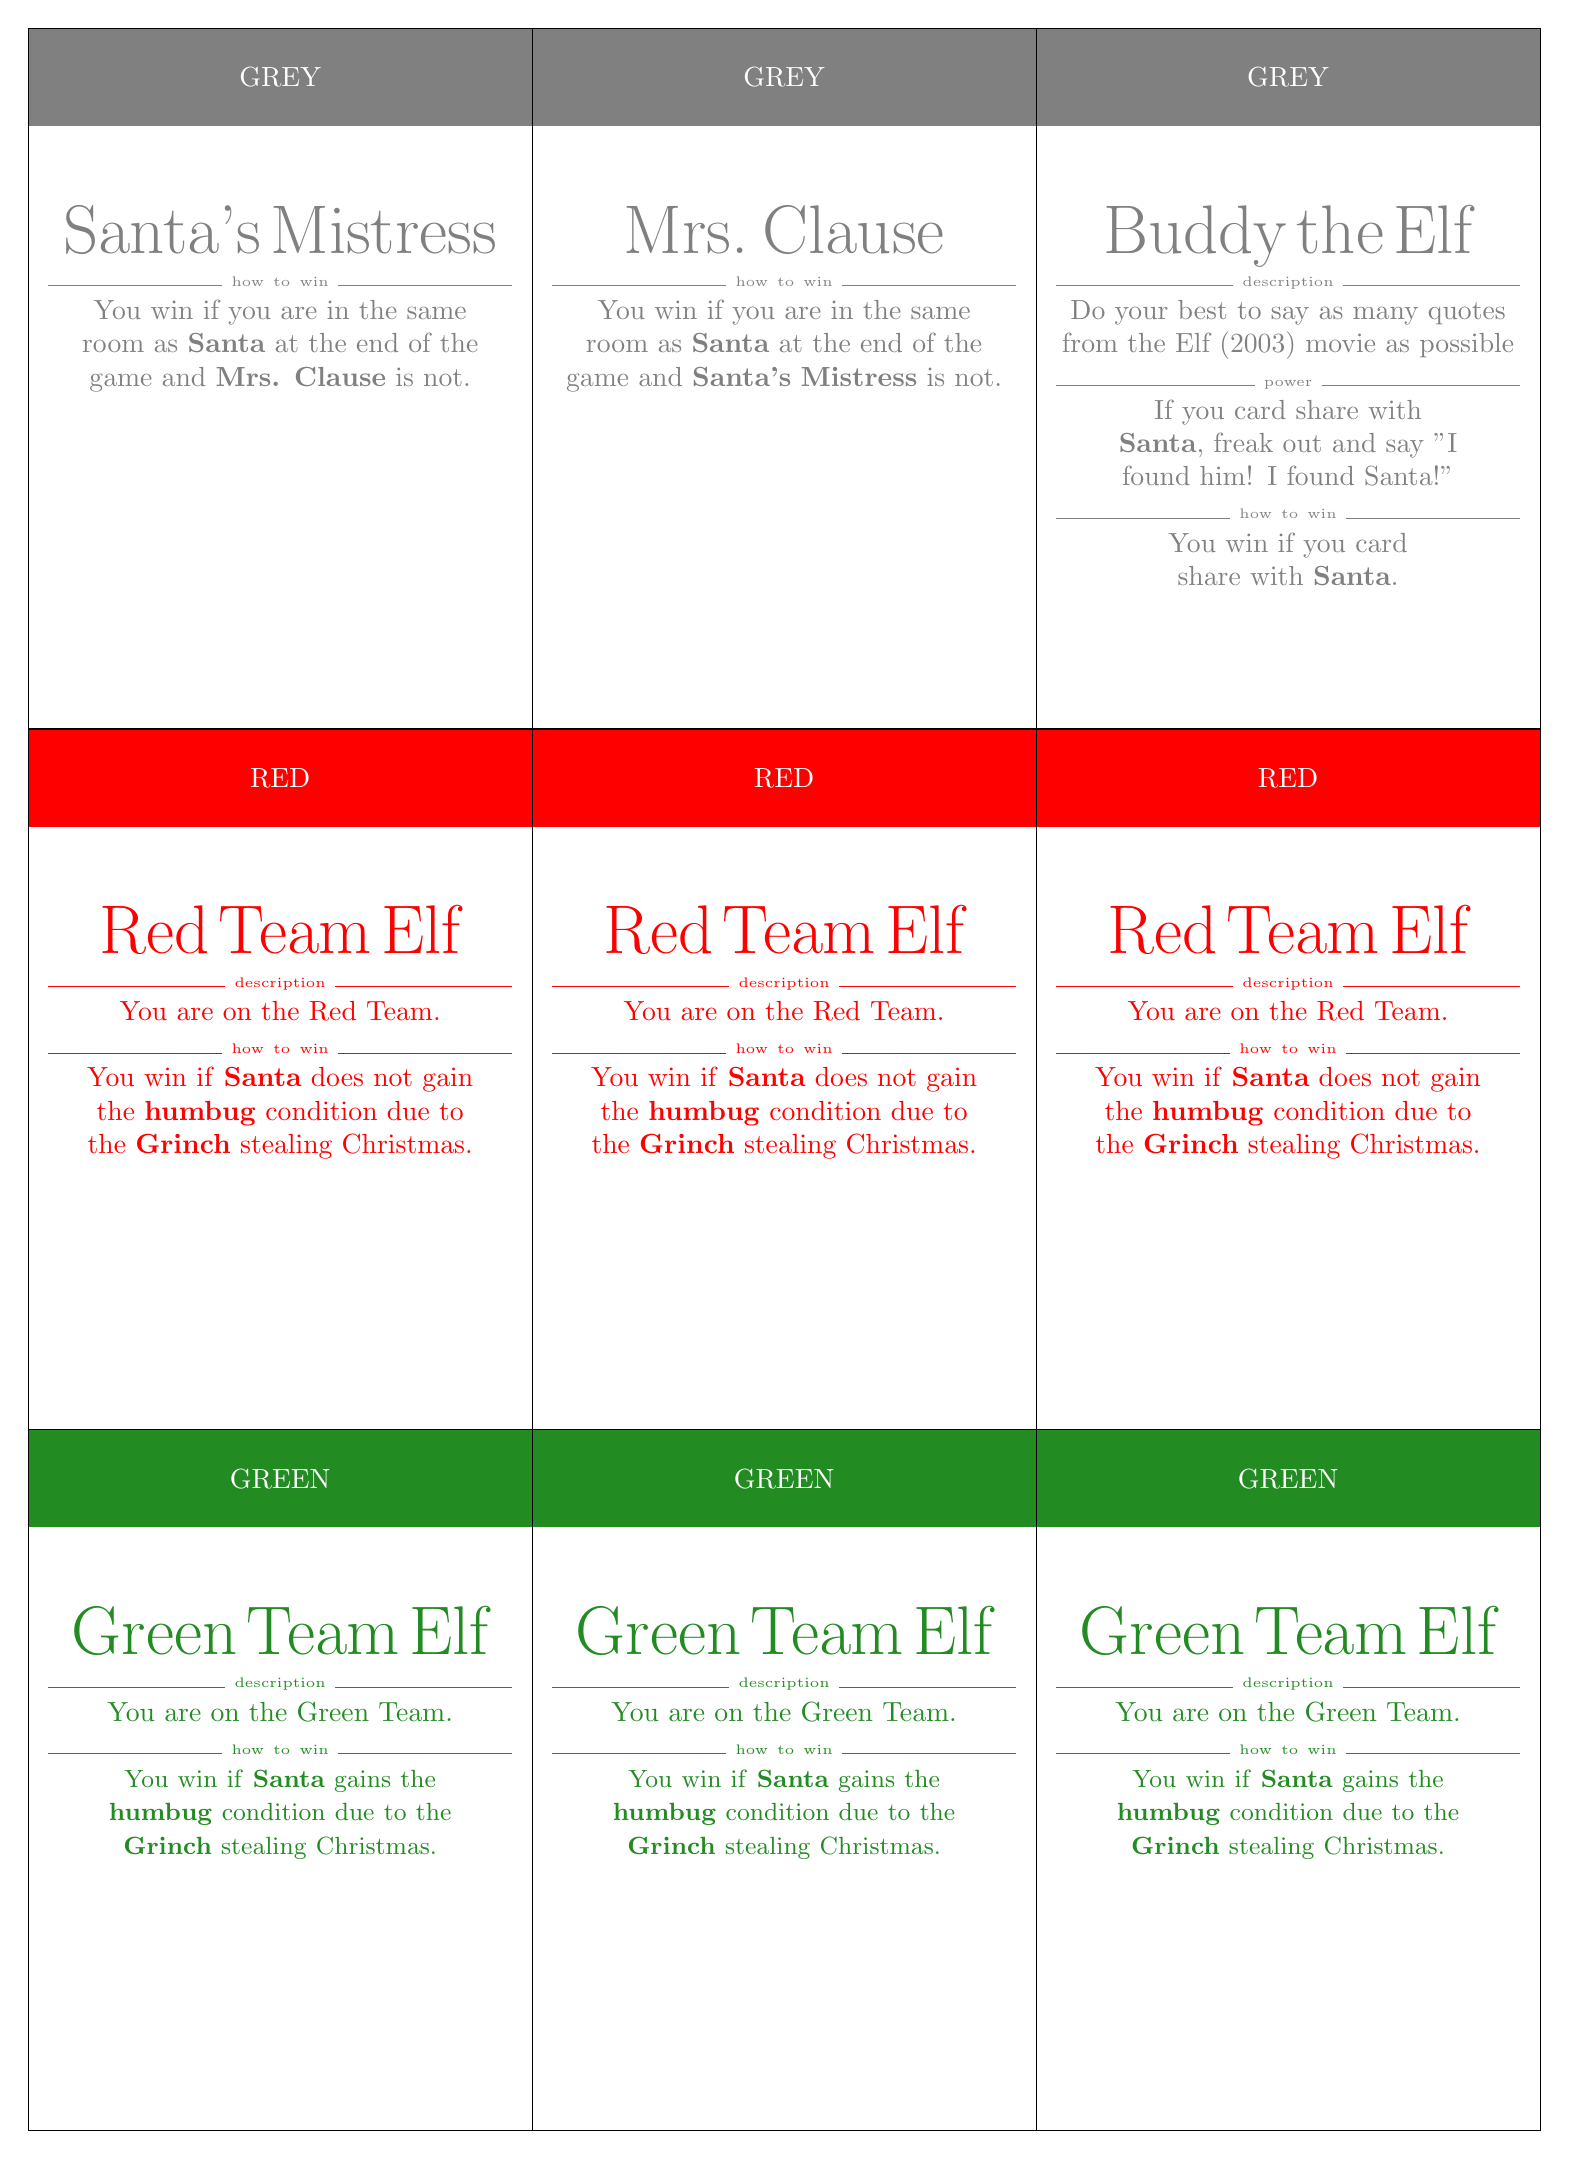
\begin{tikzpicture}[outer sep=0]

% SANTA'S MISTRESS
\node[teamshare, fill=gray] (1) at (3.2,26.7) {\HUGE GREY};
\node[cardtext, text=gray] at (3.2,24.7) {
	{\Huge Santa's Mistress}
	\\\winseperator
	You win if you are in the same room as \condition{Santa} at the end of the game and \condition{Mrs. Clause} is not.
};

% MRS. CLAUSE
\node[teamshare, fill=gray] at (9.6,26.7) {\HUGE GREY};
\node[cardtext, text=gray] at (9.6,24.7) {
	{\Huge Mrs. Clause}
	\\\winseperator
	You win if you are in the same room as \condition{Santa} at the end of the game and \condition{Santa's Mistress} is not.
};

% BUDDY THE ELF
\node[teamshare, fill=gray] at (16,26.7) {\HUGE GREY};
\node[cardtext, text=gray] at (16,24.7) {
	{\Huge Buddy the Elf}
	\\\descriptionseperator
	Do your best to say as many quotes from the Elf (2003) movie as possible
	\\\actionseperator
	If you card share with \condition{Santa}, freak out and say "I found him! I found Santa!"
	\\\winseperator
	You win if you card share with \condition{Santa}.
};
% RED TEAM ELF
\node[teamshare, fill=red] at (3.2,17.8) {\HUGE RED};
\node[cardtext, text=red] at (3.2,15.8) {
	{\Huge Red Team Elf}
	\\\descriptionseperator
	You are on the Red Team.
	\\\redwinsection
};

% RED TEAM ELF
\node[teamshare, fill=red] at (9.6,17.8) {\HUGE RED};
\node[cardtext, text=red] at (9.6,15.8) {
	{\Huge Red Team Elf}
	\\\descriptionseperator
	You are on the Red Team.
	\\\redwinsection
};

% RED TEAM ELF
\node[teamshare, fill=red] at (16,17.8) {\HUGE RED};
\node[cardtext, text=red] at (16,15.8) {
	{\Huge Red Team Elf}
	\\\descriptionseperator
	You are on the Red Team.
	\\\redwinsection
};

% GREEN TEAM ELF
\node[teamshare, fill=ForestGreen] at (3.2,8.9) {\HUGE GREEN};
\node[cardtext, text=ForestGreen] at (3.2,6.9) {
	{\Huge Green Team Elf}
	\\\descriptionseperator
	You are on the Green Team.
	\\\greenwinsection
};

% GREEN TEAM ELF
\node[teamshare, fill=ForestGreen] at (9.6,8.9) {\HUGE GREEN};
\node[cardtext, text=ForestGreen] at (9.6,6.9) {
	{\Huge Green Team Elf}
	\\\descriptionseperator
	You are on the Green Team.
	\\\greenwinsection
};

% GREEN TEAM ELF
\node[teamshare, fill=ForestGreen] at (16,8.9) {\HUGE GREEN};
\node[cardtext, text=ForestGreen] at (16,6.9) {
	{\Huge Green Team Elf}
	\\\descriptionseperator
	You are on the Green Team.
	\\\greenwinsection
};

\draw (0,0) -- (19.2,0);
\draw (0,8.9) -- (19.2,8.9);
\draw (0,17.8) -- (19.2,17.8);
\draw (0,26.7) -- (19.2,26.7);

\draw (0,0) -- (0,26.7);
\draw (6.4,0) -- (6.4,26.7);
\draw (12.8,0) -- (12.8,26.7);
\draw (19.2,0) -- (19.2,26.7);



\end{tikzpicture}

%Background is not my own. But courtesy of a user on BGG
\includepdf[pages={1}, angle=90]{cardsbackground.pdf}


\end{document}